\documentclass[twoside,10pt]{article}
\usepackage{amsmath,amsfonts,amsthm,fullpage}
\usepackage{algorithm}
\usepackage{algorithmic}
\usepackage{graphicx}


\begin{document}

\title{ISYE 6740 Spring 2021\\ Homework 1}
%\author{Yao Xie}
\date{}

\maketitle

\vspace{-.5in}

In this homework, the superscript of a symbol $\text x^i$ denotes the index of samples (not raising to $i$th power); this is a convention in this class. 



\section{$K$-means clustering [60 points]}



Given $m$ data points $\text x^i$, $i=1,\dots, m$, $K$-means clustering algorithm groups them into $k$ clusters by minimizing the distortion function over $\{ r^{ij}, \mu^j \}$
\begin{equation}
J =\sum_{i=1}^m\sum_{j=1}^k r^{ij} \|\text x^i-\mu^j\|^2,
\label{J_def}
\end{equation}
where $r^{ij}=1$ if $\text x^i$ belongs to the $j$-th cluster and $r^{ij}=0$ otherwise.

\begin{enumerate}

\item (10 points) Derive mathematically that using the squared Euclidean distance $\|\text x^i-\mu^j\|^2$ as the dissimilarity function, the centroid that minimizes the distortion function $J$  for given assignments $r^{ij}$ are given by
   $$\mu^j=\frac{\sum_i r^{ij} \text x^i}{\sum_i r^{ij}}.$$
   That is, $\mu^j$ is the center of $j$-th cluster.  \\
   Hint: You may start by taking the partial derivative of $J$ with respect to $\mu^j$, with $r^{ij}$ fixed.
   
   
\item (10 points) Derive mathematically what should be the assignment variables $r^{ij}$ be to minimize the distortion function $J$, when the centroids $\mu^j$ are fixed.
   
\item (10 points) Write down a pseudocode for $K$-means algorithm here, based on your derived results. 

\item (10 points) Explain why $K$-means algorithm converges to a local optimum in finite steps. 

\item (20 points) Calculate $k$-means by hands using Euclidean distance, i.e., the set up in Equation (\ref{J_def}).  Given $5$ data points configuration in Figure 1. Assume $k = 2$.  Assuming the initialization of centroid as shown.

\begin{enumerate}
\item (15 points) Complete the following table for all iterations until the algorithm converges.
\begin{table}[h!]
\begin{center}
\begin{tabular}{c|c|c|c|c|c|c|c}
Iteration No. & $\mu^1$ & $\mu^2$ & $r^{11}$ &  $r^{21}$ &  $r^{31}$ &  $r^{41}$ &  $r^{51}$ \\\hline
& & & &  & & &\\\hline
& & & &  & & &\\
\end{tabular}
\end{center}
\end{table}
\item (5) points How many iterations it takes for $k$-means to converge?
\end{enumerate} 

\begin{figure}[h!]
\begin{center}
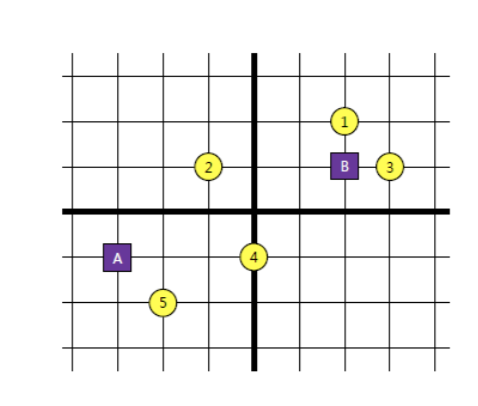
\includegraphics[width = .8\textwidth]{points.png}
\end{center}
\caption{K-means.}
\end{figure}

\end{enumerate}


\clearpage

\section{Image compression using clustering [40 points]}

In this programming assignment, you are going to apply clustering algorithms for image compression. Your task is implementing \emph{$K$-means} for this purpose.  {\bf It is required you implementing the algorithms yourself rather than calling from a package.} 


\subsubsection*{Formatting instruction}


\textbf{Input}
\begin{itemize}
  \item \texttt{pixels}: the input image representation. Each row contains one data point (pixel). For image dataset, it contains 3 columns, each column corresponding to Red, Green, and Blue component. Each component has an integer value between 0 and 255.
  \item \texttt{k}: the number of desired clusters. Too high value of $K$ may result in empty cluster error. Then, you need to reduce it.
\end{itemize}

\textbf{Output}
\begin{itemize}
  \item \texttt{class}: cluster assignment of each data point in pixels. The assignment should be 1, 2, 3, etc. For $k = 5$, for example, each cell of class should be either 1, 2, 3, 4, or 5. The output should be a column vector with \texttt{size(pixels, 1)} elements.
  \item \texttt{centroid}: location of $k$ centroids (or representatives) in your result. With images, each centroid corresponds to the representative color of each cluster. The output should be a matrix with $K$ rows and 3 columns. The range of values should be [0, 255], possibly floating point numbers.
\end{itemize}

\subsubsection*{Hand-in}
Both of your code and report will be evaluated. Upload them together as a zip file. In your report, answer to the following questions:
\begin{enumerate}
  \item (30 points) Compress pictures using $k$-means, for \texttt{beach.bmp} and \texttt{football.bmp} and also choose a third picture of your own to work on. We recommend size of $320 \times 240$ or smaller. Run your $k$-means implementation with these pictures, with several different $k = 2, 4, 8, 16$. How long does it take to converge for each $k$ (report the number of iterations, as well as actual running time)? Please write in your report, and also include the resulted compressed pictures for each $k$.
  \item (10 points) Run your $k$-means implementation with different initialization centroids. How does this it affect your final result? (We usually randomize initial location of centroids in general. To answer this question, an intentional poor assignment may be useful.) Please write in your report. 
\end{enumerate}


\subsubsection*{Note}
\begin{itemize}
  \item You may see some error message about empty clusters when you use too large $k$. Your implementation should treat this exception as well. That is, do not terminate even if you have an empty cluster, but use smaller number of clusters in that case.

  \item   We recommend you to test your code with several different pictures so that you can detect some problems that might happen occasionally. 

  \item If we detect copy from any other student's code or from the web, you will not be eligible for any credit for the entire homework, not just for the programming part. Also, directly calling built-in functions or from other package functions is not allowed.
\end{itemize}




\end{document}
